\documentclass[10pt]{article}
\usepackage[utf8]{inputenc}
\usepackage{amsmath}
\usepackage{amsfonts}
\usepackage{tikz}
\usepackage{amssymb}
%\usepackage{fullpage}
\usepackage[top=1in, bottom=1in, left=1in, right=1in]{geometry}
\usepackage{graphicx}
\usepackage{hyperref}
\usepackage{subcaption}
\usepackage{float}
\usepackage[section]{placeins}
\graphicspath{{./FigJar/}}
\begin{document}
\author{Erdem M. Karaköylü}
\title{A Bayesian Approach to OC4}
\date{\today}
\maketitle
\tableofcontents
\newpage

\newcommand{\reddash}{\raisebox{2pt}{\tikz{\draw[-,red,dashed,line width=1.2pt](0,0) -- (5mm,0);}}}
\newcommand{\blkdash}{\raisebox{2pt}{\tikz{\draw[-,black,dashed,line width=1.2pt](0,0) -- (5mm,0);}}}
\newcommand{\blksold}{\raisebox{2pt}{\tikz{\draw[-,black,solid,line width=1.2pt](0,0) -- (5mm,0);}}}

\section{Introduction}
	\subsection{Background}
		\begin{itemize}
		\item Necessity for estimating chlorophyll
		\item State of current chlorophyll algorithms
		\item Basic empirical form
		\begin{align}
		log_{10}\left(chlor_a\right) = a_0 + \sum_{i=1}^ja_ilog_{10}\left(\frac{max\left(Rrs	\left(\lambda_{blue}\right)\right)}{Rrs\left(\lambda_{green}\right)}\right)
		\end{align}
		\item Problems with current algorithms:
		\begin{itemize}
			\item collinearity of inputs
			\item poor performance in coastal
			\item maximum likelihood estimation approach $\rightarrow$ increased odds of overfitting (lack of in-situ data vailability  compared to satellite data makes it worse)
		\end{itemize}
	\end{itemize}
	\subsection{Proposed framework}
		\subsubsection{Basis reduction via PCA}
		\begin{itemize}
			\item PCA of Rrs to reduce overlap of information between predictor variables
		\end{itemize}
		\subsubsection{Bayesian framework for chlorophyll estimation from remote sensing data}
			\begin{itemize}
				\item transparent construction of models with explicit formulation of assumptions,
				\item assumptions/background information codified as priors,
				\item feasibility of priors verifiable before data collection via prior predictive checks
				\item built-in structure for selecting relevant features,
				\item posterior distribution as rich information structure from which to estimate parameter uncertainty as well as output prediction uncertainty,
				\item predictive ability of model assessed via posterior predictive checks
				\item multiple models encouraged by bayesian workflow,
				\item evaluation/comparison between models using both information about model complexity and posterior distribution (WAIC),
			\end{itemize}
		\subsubsection{Reproducibility}
			\begin{itemize}
				\item iterative process of bayesian framework relies on reproducibility for progress
				\item code available via github
				\item data available via osf
			\end{itemize}
			
%----------------- END INTRODUCTION --------------------------

\section{Methods}

	\subsection{Model Development}		
		\subsubsection{Bayesian Linear Regression}
			\begin{itemize}
				\item Order 1 regression for interpretable coefficients
				\item no interaction terms
				\item regularized horseshoe prior for feature selection
			\end{itemize}
		\subsubsection{Bayesian Linear Regression with Interaction Terms}
			\begin{itemize}
				\item generation of 1st order interaction terms
				\item allowing for both strong and weak heredity
			\end{itemize}
		\subsubsection{Bayesian Neural Network}
			\begin{itemize}
				\item Specific hierarchical structure for ARD
				\item HL1 4 NN with elu activation
			\end{itemize}
		\subsubsection{Bayesian OC4 version as Baseline}
	
	\subsection{Prior Predictive Checks}
	
	\subsection{Data Acquisition/Exploration/Transformation}
	
	\subsection{Model Fitting}
	
	\subsection{Marginal Posterior of Coefficients $\rightarrow$ Feature Relevance Determination}	
	
	\subsection{Posterior Predictive Checks}
	
	\subsection{Model Comparison Through Posterior Predictive Checks}
	
%----------------- END METHODS --------------------------

\section{Results}

%----------------- END RESULTS --------------------------


%----------------- END DISCUSSION --------------------------


	
\end{document}
			
		%	\begin{figure}[H]
		%		\centering
		%		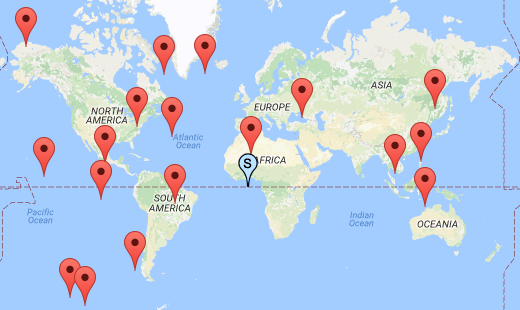
\includegraphics[scale=0.5]{randomMapPts.png}
		%		\caption{Random sampling of 18 geographic locations}
		%	\end{figure}
		